\section{Turret Test}
The turret was tested using a circular target moving at $0,19$ $m/s$ in a straight line. 
The target was moved away from the turret in 25-cm increments until the turret was unable to hit the target. Starting at 75 cm, 5 test shots were performed at each distance in both left-to-right and right-to-left direction, from the perspective of the turret. A hit or miss was noted, with no regard as to where on the target the projectile hit. The hit ratio is shown in \autoref{systest}, as a function of distance:

\begin{figure}[hbtp]
	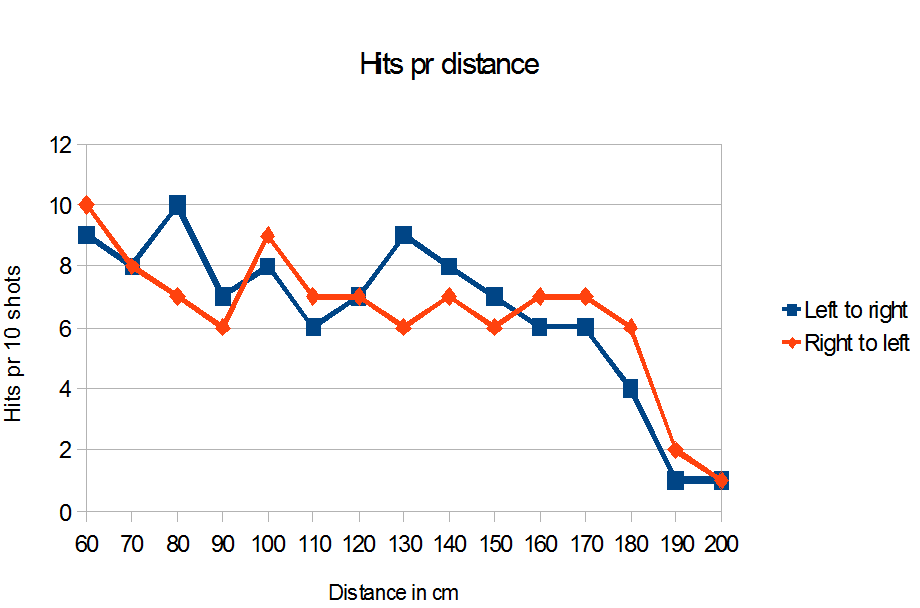
\includegraphics[scale=0.5]{img/test.png}
	\caption{Systematic test data}
	\label{systest}
\end{figure}

As can be seen the turret consistently hits the target more than half the time on the 75 - 175 cm range in the right to left direction. The highest hit to miss ratio is at 150cm, where there are only 3 hits. After 175 cm, which was the predicted maximum range for these intervals, the turret is not physically able to hit the target at all in either direction. The accuracy of the turret fluctuates, but variances in hits are put down to inaccuracies in placement of Kinect relative to turret and in detecting the target correctly. Overall the right to left moving target is hit more consistently than the left to right moving target (ignoring the 200 cm data, 88\% relative to 64\%). This is due to the Kinect's varying ability to identify the target properly, which is more pronounced when the target is moving from the left to the right.

The overall hit percent in both directions, ignoring the 200 cm data, is 76\%.
